%% bare_jrnl.tex
%% V1.4b
%% 2015/08/26
%% by Michael Shell
%% see http://www.michaelshell.org/
%% for current contact information.
%%
%% This is a skeleton file demonstrating the use of IEEEtran.cls
%% (requires IEEEtran.cls version 1.8b or later) with an IEEE
%% journal paper.
%%
%% Support sites:
%% http://www.michaelshell.org/tex/ieeetran/
%% http://www.ctan.org/pkg/ieeetran
%% and
%% http://www.ieee.org/

%%*************************************************************************
%% Legal Notice:
%% This code is offered as-is without any warranty either expressed or
%% implied; without even the implied warranty of MERCHANTABILITY or
%% FITNESS FOR A PARTICULAR PURPOSE! 
%% User assumes all risk.
%% In no event shall the IEEE or any contributor to this code be liable for
%% any damages or losses, including, but not limited to, incidental,
%% consequential, or any other damages, resulting from the use or misuse
%% of any information contained here.
%%
%% All comments are the opinions of their respective authors and are not
%% necessarily endorsed by the IEEE.
%%
%% This work is distributed under the LaTeX Project Public License (LPPL)
%% ( http://www.latex-project.org/ ) version 1.3, and may be freely used,
%% distributed and modified. A copy of the LPPL, version 1.3, is included
%% in the base LaTeX documentation of all distributions of LaTeX released
%% 2003/12/01 or later.
%% Retain all contribution notices and credits.
%% ** Modified files should be clearly indicated as such, including  **
%% ** renaming them and changing author support contact information. **
%%*************************************************************************


% *** Authors should verify (and, if needed, correct) their LaTeX system  ***
% *** with the testflow diagnostic prior to trusting their LaTeX platform ***
% *** with production work. The IEEE's font choices and paper sizes can   ***
% *** trigger bugs that do not appear when using other class files.       ***                          ***
% The testflow support page is at:
% http://www.michaelshell.org/tex/testflow/



\documentclass[journal]{IEEEtran}
\usepackage{graphicx}
\usepackage{float}

%
% If IEEEtran.cls has not been installed into the LaTeX system files,
% manually specify the path to it like:
% \documentclass[journal]{../sty/IEEEtran}





% Some very useful LaTeX packages include:
% (uncomment the ones you want to load)


% *** MISC UTILITY PACKAGES ***
%
%\usepackage{ifpdf}
% Heiko Oberdiek's ifpdf.sty is very useful if you need conditional
% compilation based on whether the output is pdf or dvi.
% usage:
% \ifpdf
%   % pdf code
% \else
%   % dvi code
% \fi
% The latest version of ifpdf.sty can be obtained from:
% http://www.ctan.org/pkg/ifpdf
% Also, note that IEEEtran.cls V1.7 and later provides a builtin
% \ifCLASSINFOpdf conditional that works the same way.
% When switching from latex to pdflatex and vice-versa, the compiler may
% have to be run twice to clear warning/error messages.






% *** CITATION PACKAGES ***
%
%\usepackage{cite}
% cite.sty was written by Donald Arseneau
% V1.6 and later of IEEEtran pre-defines the format of the cite.sty package
% \cite{} output to follow that of the IEEE. Loading the cite package will
% result in citation numbers being automatically sorted and properly
% "compressed/ranged". e.g., [1], [9], [2], [7], [5], [6] without using
% cite.sty will become [1], [2], [5]--[7], [9] using cite.sty. cite.sty's
% \cite will automatically add leading space, if needed. Use cite.sty's
% noadjust option (cite.sty V3.8 and later) if you want to turn this off
% such as if a citation ever needs to be enclosed in parenthesis.
% cite.sty is already installed on most LaTeX systems. Be sure and use
% version 5.0 (2009-03-20) and later if using hyperref.sty.
% The latest version can be obtained at:
% http://www.ctan.org/pkg/cite
% The documentation is contained in the cite.sty file itself.






% *** GRAPHICS RELATED PACKAGES ***
%
\ifCLASSINFOpdf
  % \usepackage[pdftex]{graphicx}
  % declare the path(s) where your graphic files are
  % \graphicspath{{../pdf/}{../jpeg/}}
  % and their extensions so you won't have to specify these with
  % every instance of \includegraphics
  % \DeclareGraphicsExtensions{.pdf,.jpeg,.png}
\else
  % or other class option (dvipsone, dvipdf, if not using dvips). graphicx
  % will default to the driver specified in the system graphics.cfg if no
  % driver is specified.
  % \usepackage[dvips]{graphicx}
  % declare the path(s) where your graphic files are
  % \graphicspath{{../eps/}}
  % and their extensions so you won't have to specify these with
  % every instance of \includegraphics
  % \DeclareGraphicsExtensions{.eps}
\fi
% graphicx was written by David Carlisle and Sebastian Rahtz. It is
% required if you want graphics, photos, etc. graphicx.sty is already
% installed on most LaTeX systems. The latest version and documentation
% can be obtained at: 
% http://www.ctan.org/pkg/graphicx
% Another good source of documentation is "Using Imported Graphics in
% LaTeX2e" by Keith Reckdahl which can be found at:
% http://www.ctan.org/pkg/epslatex
%
% latex, and pdflatex in dvi mode, support graphics in encapsulated
% postscript (.eps) format. pdflatex in pdf mode supports graphics
% in .pdf, .jpeg, .png and .mps (metapost) formats. Users should ensure
% that all non-photo figures use a vector format (.eps, .pdf, .mps) and
% not a bitmapped formats (.jpeg, .png). The IEEE frowns on bitmapped formats
% which can result in "jaggedy"/blurry rendering of lines and letters as
% well as large increases in file sizes.
%
% You can find documentation about the pdfTeX application at:
% http://www.tug.org/applications/pdftex





% *** MATH PACKAGES ***
%
%\usepackage{amsmath}
% A popular package from the American Mathematical Society that provides
% many useful and powerful commands for dealing with mathematics.
%
% Note that the amsmath package sets \interdisplaylinepenalty to 10000
% thus preventing page breaks from occurring within multiline equations. Use:
%\interdisplaylinepenalty=2500
% after loading amsmath to restore such page breaks as IEEEtran.cls normally
% does. amsmath.sty is already installed on most LaTeX systems. The latest
% version and documentation can be obtained at:
% http://www.ctan.org/pkg/amsmath





% *** SPECIALIZED LIST PACKAGES ***
%
%\usepackage{algorithmic}
% algorithmic.sty was written by Peter Williams and Rogerio Brito.
% This package provides an algorithmic environment fo describing algorithms.
% You can use the algorithmic environment in-text or within a figure
% environment to provide for a floating algorithm. Do NOT use the algorithm
% floating environment provided by algorithm.sty (by the same authors) or
% algorithm2e.sty (by Christophe Fiorio) as the IEEE does not use dedicated
% algorithm float types and packages that provide these will not provide
% correct IEEE style captions. The latest version and documentation of
% algorithmic.sty can be obtained at:
% http://www.ctan.org/pkg/algorithms
% Also of interest may be the (relatively newer and more customizable)
% algorithmicx.sty package by Szasz Janos:
% http://www.ctan.org/pkg/algorithmicx




% *** ALIGNMENT PACKAGES ***
%
%\usepackage{array}
% Frank Mittelbach's and David Carlisle's array.sty patches and improves
% the standard LaTeX2e array and tabular environments to provide better
% appearance and additional user controls. As the default LaTeX2e table
% generation code is lacking to the point of almost being broken with
% respect to the quality of the end results, all users are strongly
% advised to use an enhanced (at the very least that provided by array.sty)
% set of table tools. array.sty is already installed on most systems. The
% latest version and documentation can be obtained at:
% http://www.ctan.org/pkg/array


% IEEEtran contains the IEEEeqnarray family of commands that can be used to
% generate multiline equations as well as matrices, tables, etc., of high
% quality.




% *** SUBFIGURE PACKAGES ***
%\ifCLASSOPTIONcompsoc
%  \usepackage[caption=false,font=normalsize,labelfont=sf,textfont=sf]{subfig}
%\else
%  \usepackage[caption=false,font=footnotesize]{subfig}
%\fi
% subfig.sty, written by Steven Douglas Cochran, is the modern replacement
% for subfigure.sty, the latter of which is no longer maintained and is
% incompatible with some LaTeX packages including fixltx2e. However,
% subfig.sty requires and automatically loads Axel Sommerfeldt's caption.sty
% which will override IEEEtran.cls' handling of captions and this will result
% in non-IEEE style figure/table captions. To prevent this problem, be sure
% and invoke subfig.sty's "caption=false" package option (available since
% subfig.sty version 1.3, 2005/06/28) as this is will preserve IEEEtran.cls
% handling of captions.
% Note that the Computer Society format requires a larger sans serif font
% than the serif footnote size font used in traditional IEEE formatting
% and thus the need to invoke different subfig.sty package options depending
% on whether compsoc mode has been enabled.
%
% The latest version and documentation of subfig.sty can be obtained at:
% http://www.ctan.org/pkg/subfig




% *** FLOAT PACKAGES ***
%
%\usepackage{fixltx2e}
% fixltx2e, the successor to the earlier fix2col.sty, was written by
% Frank Mittelbach and David Carlisle. This package corrects a few problems
% in the LaTeX2e kernel, the most notable of which is that in current
% LaTeX2e releases, the ordering of single and double column floats is not
% guaranteed to be preserved. Thus, an unpatched LaTeX2e can allow a
% single column figure to be placed prior to an earlier double column
% figure.
% Be aware that LaTeX2e kernels dated 2015 and later have fixltx2e.sty's
% corrections already built into the system in which case a warning will
% be issued if an attempt is made to load fixltx2e.sty as it is no longer
% needed.
% The latest version and documentation can be found at:
% http://www.ctan.org/pkg/fixltx2e


%\usepackage{stfloats}
% stfloats.sty was written by Sigitas Tolusis. This package gives LaTeX2e
% the ability to do double column floats at the bottom of the page as well
% as the top. (e.g., "\begin{figure*}[!b]" is not normally possible in
% LaTeX2e). It also provides a command:
%\fnbelowfloat
% to enable the placement of footnotes below bottom floats (the standard
% LaTeX2e kernel puts them above bottom floats). This is an invasive package
% which rewrites many portions of the LaTeX2e float routines. It may not work
% with other packages that modify the LaTeX2e float routines. The latest
% version and documentation can be obtained at:
% http://www.ctan.org/pkg/stfloats
% Do not use the stfloats baselinefloat ability as the IEEE does not allow
% \baselineskip to stretch. Authors submitting work to the IEEE should note
% that the IEEE rarely uses double column equations and that authors should try
% to avoid such use. Do not be tempted to use the cuted.sty or midfloat.sty
% packages (also by Sigitas Tolusis) as the IEEE does not format its papers in
% such ways.
% Do not attempt to use stfloats with fixltx2e as they are incompatible.
% Instead, use Morten Hogholm'a dblfloatfix which combines the features
% of both fixltx2e and stfloats:
%
% \usepackage{dblfloatfix}
% The latest version can be found at:
% http://www.ctan.org/pkg/dblfloatfix




%\ifCLASSOPTIONcaptionsoff
%  \usepackage[nomarkers]{endfloat}
% \let\MYoriglatexcaption\caption
% \renewcommand{\caption}[2][\relax]{\MYoriglatexcaption[#2]{#2}}
%\fi
% endfloat.sty was written by James Darrell McCauley, Jeff Goldberg and 
% Axel Sommerfeldt. This package may be useful when used in conjunction with 
% IEEEtran.cls'  captionsoff option. Some IEEE journals/societies require that
% submissions have lists of figures/tables at the end of the paper and that
% figures/tables without any captions are placed on a page by themselves at
% the end of the document. If needed, the draftcls IEEEtran class option or
% \CLASSINPUTbaselinestretch interface can be used to increase the line
% spacing as well. Be sure and use the nomarkers option of endfloat to
% prevent endfloat from "marking" where the figures would have been placed
% in the text. The two hack lines of code above are a slight modification of
% that suggested by in the endfloat docs (section 8.4.1) to ensure that
% the full captions always appear in the list of figures/tables - even if
% the user used the short optional argument of \caption[]{}.
% IEEE papers do not typically make use of \caption[]'s optional argument,
% so this should not be an issue. A similar trick can be used to disable
% captions of packages such as subfig.sty that lack options to turn off
% the subcaptions:
% For subfig.sty:
% \let\MYorigsubfloat\subfloat
% \renewcommand{\subfloat}[2][\relax]{\MYorigsubfloat[]{#2}}
% However, the above trick will not work if both optional arguments of
% the \subfloat command are used. Furthermore, there needs to be a
% description of each subfigure *somewhere* and endfloat does not add
% subfigure captions to its list of figures. Thus, the best approach is to
% avoid the use of subfigure captions (many IEEE journals avoid them anyway)
% and instead reference/explain all the subfigures within the main caption.
% The latest version of endfloat.sty and its documentation can obtained at:
% http://www.ctan.org/pkg/endfloat
%
% The IEEEtran \ifCLASSOPTIONcaptionsoff conditional can also be used
% later in the document, say, to conditionally put the References on a 
% page by themselves.




% *** PDF, URL AND HYPERLINK PACKAGES ***
%
%\usepackage{url}
% url.sty was written by Donald Arseneau. It provides better support for
% handling and breaking URLs. url.sty is already installed on most LaTeX
% systems. The latest version and documentation can be obtained at:
% http://www.ctan.org/pkg/url
% Basically, \url{my_url_here}.




% *** Do not adjust lengths that control margins, column widths, etc. ***
% *** Do not use packages that alter fonts (such as pslatex).         ***
% There should be no need to do such things with IEEEtran.cls V1.6 and later.
% (Unless specifically asked to do so by the journal or conference you plan
% to submit to, of course. )


% correct bad hyphenation here
\hyphenation{op-tical net-works semi-conduc-tor}


\begin{document}
\title{Research Design II }

\author{Matthew Micallef\\
Institute Of ICT\\
Malta College of Arts Science and Technology}

% note the % following the last \IEEEmembership and also \thanks - 
% these prevent an unwanted space from occurring between the last author name
% and the end of the author line. i.e., if you had this:
% 
% \author{....lastname \thanks{...} \thanks{...} }
%                     ^------------^------------^----Do not want these spaces!
%
% a space would be appended to the last name and could cause every name on that
% line to be shifted left slightly. This is one of those "LaTeX things". For
% instance, "\textbf{A} \textbf{B}" will typeset as "A B" not "AB". To get
% "AB" then you have to do: "\textbf{A}\textbf{B}"
% \thanks is no different in this regard, so shield the last } of each \thanks
% that ends a line with a % and do not let a space in before the next \thanks.
% Spaces after \IEEEmembership other than the last one are OK (and needed) as
% you are supposed to have spaces between the names. For what it is worth,
% this is a minor point as most people would not even notice if the said evil
% space somehow managed to creep in.



% The paper headers

% The only time the second header will appear is for the odd numbered pages
% after the title page when using the twoside option.
% 
% *** Note that you probably will NOT want to include the author's ***
% *** name in the headers of peer review papers.                   ***
% You can use \ifCLASSOPTIONpeerreview for conditional compilation here if
% you desire.




% If you want to put a publisher's ID mark on the page you can do it like
% this:
%\IEEEpubid{0000--0000/00\$00.00~\copyright~2015 IEEE}
% Remember, if you use this you must call \IEEEpubidadjcol in the second
% column for its text to clear the IEEEpubid mark.



% use for special paper notices
%\IEEEspecialpapernotice{(Invited Paper)}





% make the title area
\maketitle

% As a general rule, do not put math, special symbols or citations
% in the abstract or keywords.
\begin{abstract}
The increase of effectiveness of both Artificial intelligence (AI) and Machine learning (ML) have have changed the field of image processing and image recognition.The paper goes over the implementation and the testing of Local Binary Patterns Histograms (LBPH) algorithm in a face recognition system. With the aim to use this technology to eliminate the need for the use of a physical key to enter a house. 
\end{abstract}

% For peer review papers, you can put extra information on the cover
% page as needed:
% \ifCLASSOPTIONpeerreview
% \begin{center} \bfseries EDICS Category: 3-BBND \end{center}
% \fi
%
% For peerreview papers, this IEEEtran command inserts a page break and
% creates the second title. It will be ignored for other modes.
\IEEEpeerreviewmaketitle


\section{Introduction}

\IEEEPARstart{T}{he} proposed system uses a Haar cascade classifier to detect faces, a Local Binary Patterns Histograms (LBPH) algorithm for face recognition, and a Raspberry Pi camera for real-time video capturing. The ultimate goal for the research carried out is to evaluate the feasibility of using the above mentioned technologies as a cost-effective and secure home entry solution in replacement of a conventional lock and key. The rational behind researching this topic is due to flaws with traditional security measures which include, the need for a key, the chance of the key being lost or stolen or even forgotten  in the premise, these flaws all lead to the same scenario the user being unable to enter the home.\\ Facial recognition has been emerging more and more as a technology and should be further investigated in the above use case due to its non-transferability which climates the loss of the key in the traditional security system and also the convenience, the user can never be locked out of the house cause his face now the replacement key is always available. This paper goes through fundamental aspects such as the number of training images required for reliable facial recognition, more over it goes through the effect of using gray scale images.\\
The paper positions itself within two major areas of studies it basis itself on computer vision and also practical home security solutions, it is set apart from the vast majority of studies that research facial recognition by the use of accessible hardware in this case the raspberry pi four and the raspberry pi camera thus extending to the more cost effective smart home solution rather than a purely academic or high-end applications of facial recognition.\\
The hypothesis for this research is the integration of a Haar cascade classifier, an LBPH algorithm, and a Raspberry Pi four and Pi camera to potentially create a superior form of entry to unlocking a lock without using a key in the aim of make it being more secure, affordable and user convenient.\\
\\

\subsection{Research Approach}

The research being carried out will follow a systematic approach based on a Research Onion depicted in the appendices [Figure 1]. The Layers to the research oinon are explained below 

\begin{enumerate}
  \item Research Philosophy: The study concentrates on observable phenomena which utilizes a structured and organised methodology and thus follows a Positivism Philosophy 
  \item Research Approaches: Due to the study using  established theories and research carried out in the domain of facial recognition and the LBPH algorithm, the paper will follow a Deductive approach.
  \item Research Strategy: The strategy could be classified as an experiment due to having a devised a system and are adjusting a factor which is the quantity of training images to examine the influence on the system's effectiveness.
  \item Research Choices: The research adopts a mono-method, by the use of quantitative data gathered from testing the system.
  \item Time Horizons: The research is conducted over a specific point in time rather than longitudinal and thus being cross-sectional.
  \item Techniques and Procedures: The data being collected involves testing the facial recognition sysyem under different conditions and collecting statistical data. Data that will investigate the correlation between the number of training images and the systems performance.
\end{enumerate}



\section{Literature Review}
\IEEEPARstart{T}{he} methodology undertaken in this paper is based on the integration and the implementation of different technologies to identify an alternative home entry solution.\\

A Haar cascade classifier is a machine learning object detection method which is used to identify objects in an image or video. This classifier is trained based on both positive and negative images of the object to be recognized. Calculable rectangular features are used to detect the presence of the object being recognized in the image, these are also known as Haar features[1]. The cascading aspect for this classifier refers to a number of increasingly complex classifiers that reject negative samples to primarily focus the processing resources on more promising areas of the image.\\


The Local Binary Patterns Histograms (LBPH) algorithm is used in image processing and pattern recognition due to it being a powerful feature extractor, this algorithm is mainly used for facial recognition applications. This algorithm works by comparing each pixel in the image with its neighboring pixels it encodes the resulting relationship into a binary pattern theses patterns can then be used to create histograms that can be used for image comparison and other recognition tasks.A representation of how 
the LBPH algorithm works can be seen in the below figure (Fig 1).

\begin{figure}[H]
    \centering
    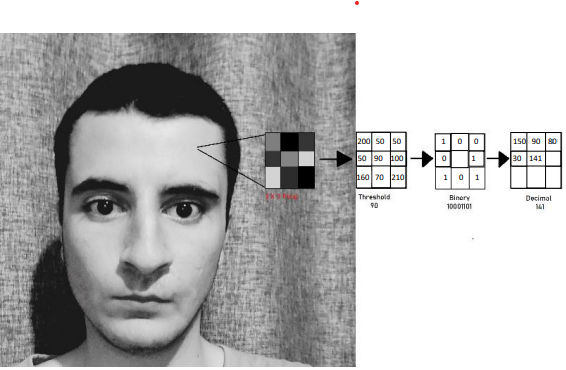
\includegraphics[width=\columnwidth]{./images/Figure1.png}
    \caption{Conversion of a Gray-scale image to decimal}
    \label{fig:my_label}
\end{figure}

A raspberry pi is a small and affordable single board computer. It is based on a Quad core 64-bit ARM-Cortex A72 which runs at 1.5GHz and the model which was used in the research carried out was equipped with 4Gb of RAM. This not only classifies the board as affordable but only has good performing hardware.\\

Their are similar studies that use a raspberry pi for facial recognition, one paper uses a raspberry pi connected to a web cam, passive infrared (PIR) sensor and uses the OpenCV library for image processing, the aim of this study was to use the PIR sensor to identify movement in the room and to trigger the web camera to start transmitting images to a cascade classifier to look for facial features to detect a person[2].\\

Another research paper went into more depth, two models were evaluated for use these are the Haar cascade classifier and also the Histogram of Oriented Gradients (HOG), the evaluation for the Haar model used Adaboost training which selected the best features to form a better classifier. An HOG model uses histograms to represent the distribution of pixel intensities in an image. This algorithm divides the given image into 8 * 8 cells and a histogram for each cell is generated, normalization takes place over a larger 16*16 cell to make the descriptor insensitive to lighting variations. All vectors from each block are concatenated into one vector to form the final HOG feature vector. The latter HOG algorithm explained above was was found to be too computationally intensive for the Raspberry Pi 3 Model B+ and was implemented using a system with an i5 CPU which also deemed to be too computationally intense for [3].\\

A different research paper uses a similar approach to the one that was undertaken it uses a raspberry pi zero a more affordable model by the Pi foundation and a web cam wich although the model is not stated the resolution is said to be more or equal to 720p. A data set of four individual was created with each individual having 10 images in a different environment, the process of creating a trainer file was done through a python script which loaded the images into grayscale and subsequently into a Numpy array. The Haar Cascade frontal face classifier was used to detect a face in the images provided and each image was appended with a respective id. A model was trained using the trainer file generated and the LBPH algorithm being executed on the raspberry pi uses this model for facial recognition. The study also examined the size and loading time for the trainer file by varying the number of images for each of the four users[4].\\

In both the above studies they use Haar classifier although the research carried out by Singh et al, goes a step further to integrate Adaboost which should help to to construct a stronger classifier than that of Negpal et al, the use of the better Raspberry pi 3 should slo make training and facial recognition faster due to the better hardware.\\

in the study carried out by Mladenova et al, a similar approch was taken with the aim to open locker doors in an airport by means of a raspberry pi 3 and the use of a Principal Component Analysis (PCA) as a dimensionality reduction algorithm, this was done in order to simplify the the process of comparing facial images. The algorithm treats each image inputted as a one dimensional feature vector created from the pixel values of the image. PCA reduces the non-informative parts while preserving the most informative aspects of the image this is done to reduce the dimension of the feature vectors. In facial recognition, the use of PCA is known as the Eigenfaces method this involves representing the faces as a smaller collection f the key features, these are said to be the principal components of the collection of face images, this makes the comparison between the faces slightly more computationally manageable[5].\\

When comparing the three main approaches above two of the papers follow a similar flow by the use of a combination of a Convolutional Neural Networks (CNN) and Recurrent Neural Networks (RNN) for face recognition, this approach basis itself on deep learning models which are better able to learn complex patterns in the input data. CNN helps to adaptive and automatically learn spatial hierarchies of features, while RNN helps in learning  temporal dependencies in the data. Although this method of facial recognition gives high accuracy it requires a substantial amount of computational resources and a lot of training data. On the other hand the research carried out by Mladenova et al, uses PCA for feature selection and dimensional reduction. Although this approach is less resource intensive in terms of computational resources, this approach could lead to lower accuracy when compared to the above two research papers discussed above more particularly when it comes to complex patterns in the data set.

The following Conference paper written by Nikita et al, uses a different hardware approach that the four other studies discussed above it uses an Arduino based hardware solution rather than a raspberry pi but ultimately they are both affordable single board computers. The implementation captures a video input stream and uses a motion detection module that is written in MATLAB. if motion is detected the frame that motion was detected on is passed through to a facial detection module also written in MATLAB. if this module identifies facial features, the coordinates of the faces and also the frame is sent to a facial recognition module, which uses the coordinates to extract the faces from the frame. The following toolboxes are used in terms of software imported from MATLAB, the Computer Vision Toolbox, the Statistical Toolbox and the image acquisition tool box.\\

The facial recognition process is based on PCA using the Eigen faces method similar to the approach taken by Mladenova et al, where the system creates a training set of face images, then separates the frames down to individual vectors, A covariance matrix is formed, from which the eigenfaces better known as eigenvectors are derived. The system focuses on the key facial attributes rather than the entire facial data set to be able to best determine the weights of each frame that it is processing. it than uses the weights of the new face image and compares it the weights of the images that it has stored in a database.\\

The Euclidean Distance (ED) method is used for classification, with the maximum threshold set to $4.00 \times 10^{15}$. If the ED difference is greater than the above set threshold the classifier will fail to recognize the individuals identity. The above classifier is given eight images of the user to be trained on compared to the ten images that Negpai et al used.\\

All the implementations given above use a different method and algorithm for facial recognition the first three implementations rely on various deep learning techniques with different loss functions and different data preparation stages. The last two implantation's use a simpler yet still effective method of facial recognition by means of PCA. The dependent factor on choosing any of these implementations relays on the specific computational resources that the system has to offer that the margin of acceptable error rate.\\

A Literature Map is attached in the appendices section [Fig 3] to gather insight of how research was mapped out.


\section{Methodology}
To address the hypothesis these objectives and research questions where identified.\\
Objectives
\begin{enumerate}
  \item To dynamically create a dataset based on facial features.
  \item To implement an efficient face detection mechanism using Haar cascade classifier.
  \item To apply an effective facial recognition algorithm using LBPH.
  \item To determine the optimal number of training images for high accuracy. 
  \item To evaluate the feasibility and safety of the technology for practical use.
\end{enumerate}
Research questions 
\begin{enumerate}
  \item What kind of data set is required for detecting faces?
  \item What algorithm can be used to best distinguish between faces?
  \item Is there any difference in the confidence levels when increasing the number of images taken for each new individual?
  \item Is it safe to adopt this technology for the above mentioned use case? 
\end{enumerate}

The following subsequent stages will be used to carry out the execution of the research paper.

\begin{enumerate}
  \item The first stage of the Development process would be to gather the initial user data, the data that will be used to train a model with. A mechanism for the user to enter their name is created and a sequence of images is subsequently taken.
  \item The images are then collected converted to gray scale and saved in a folder structure using a new given id 
  \item A Haar cascade classifier will then be used to identify weather their is a face in the image or not and the image will than be cropped and the original image taken will be overwritten by the cropped image of the users face.
  \item An LBPH algorithm will be used to train a model based on the images that were gathered and processed.
  \item The model will then be automatically be used to start recognizing users that are in front of the raspberry pi camera.
  \item The model will then be tested with different amounts of training images to understand the correlation between the number of images taken for each new individual.
  \item A comprehensive review of the results should be undertaken to identify weather or not this implementation can be deployed as a product, due to the known potential for high false positives/negatives that the LBPH model can generate.
\end{enumerate}

\subsection{Data Set}
In the context of this implementation, their is no need for a pre-existing data set, the reason being is that the model training is being based on the individuals who have been granted entry to the home. As mentioned above whenever a new user is allowed entry to the home, a number of images are taken and stored the latter being that the images contains a face, upon the images being saved in the particular structure the model will get retrained and the new user will now be recognised by the model in conjunction with the existing users that the model has already been trained on. The above described operation can be executed effortlessly, in the scenario that a user is no longer granted entry to the home, the images of that particular user can be purged and the model can be retrained and as a result the model will no longer recognise the user.

\subsection{Face Trainer}
To asses the presence of a face in the provided image, the Frontal face  Haar classifier this classifier was chosen for it being fast in execution, having a high accuracy, and minimal false positives. This classifier is trained using a number of different images which includes images with a face vi-sable and without, different skin tones, identifying eyes and facial structure.

\subsection{Facial recognition}
The Open CV library was chosen for it being open-source and has three built in facial recognition algorithms which include the  Eigenfaces, Fisherfaces and the
LBPH. The LBPH algorithm when compared to the above mentioned algorithms can not only recognise the front of the faces but also the sides of the face which makes this algorithm a better option in this particular use case.

\subsection{Number of images}
The number of images used in the initial stage of this implementation will be tested to see the affect of the number of images that the LBPH algorithm is trained on, this would be done to identify a number of images which offer a high accuracy without sacrificing storage space, also with reducing the number of images that the model is trained on the retraining of the model will be faster given the less images that the model needs to train on both for existing users and the user that is being added.

\subsection{Research Philosophy and Approach}
The research follows a positive philosophical approach given that Facial recognition is in essence a quantitative problem, involving precise measurements of facial features and characteristics computed through mathematical formulae. Based on this approach the research utilized the deductive approach to establish a hypothesis and test it through the methodology described.
\\
The experimental research strategy was used to focus on the correlation between the number of images used for training and the resulting model's accuracy. The mono -method will be used, relying mainly on quantitative data to potentially provide precise, numerical data which is beneficial for statistical analysis in the field of facial recognition.
\\The above research philosophies were used to fulfil the research objectives outlined above, but to also provide substantiated knowledge to implement facial recognition technology in the given context.
\subsection{Method of Analysis}
The performance of the facial recognition model will be assessed based on the confidence level it exhibits when identifying individuals, this method was chosen to mimic the intended task in correctly identifying individuals. By using the confidence level, the model can be assessed based on the correct identification but also on the certainty that the model has in the identification.

\subsection{Ethical Considerations}
Due to the nature of facial recognition and the need for collecting and analysing potentially sensitive data these ethical considerations are being taken into consoderation 

\begin{enumerate}
  \item Informed Consent: Before any data is collected the user should be informed and given the option to accept and deny the capturing of their images for the use case.
  \item Data Protection and Privacy: To ensure data anonymity the user data will be stored based on an id and security measures like data encryption are used 
  \item Compliance with Regulations: The research will comply with all the relevant data protection regulations such as the General Data Protection Regulation (GDPR) in the European Union. Meaning that the data collected will be processed only for the process of facial recognition and will not be retained for more than necessary.
\end{enumerate}



future improvements possible conc

For robust and reliable facial recognition, ensure you collect images under various conditions such as different lighting, angles, expressions, etc.

% An example of a floating figure using the graphicx package.
% Note that \label must occur AFTER (or within) \caption.
% For figures, \caption should occur after the \includegraphics.
% Note that IEEEtran v1.7 and later has special internal code that
% is designed to preserve the operation of \label within \caption
% even when the captionsoff option is in effect. However, because
% of issues like this, it may be the safest practice to put all your
% \label just after \caption rather than within \caption{}.
%
% Reminder: the "draftcls" or "draftclsnofoot", not "draft", class
% option should be used if it is desired that the figures are to be
% displayed while in draft mode.
%
%\begin{figure}[!t]
%\centering
%\includegraphics[width=2.5in]{myfigure}
% where an .eps filename suffix will be assumed under latex, 
% and a .pdf suffix will be assumed for pdflatex; or what has been declared
% via \DeclareGraphicsExtensions.
%\caption{Simulation results for the network.}
%\label{fig_sim}
%\end{figure}

% Note that the IEEE typically puts floats only at the top, even when this
% results in a large percentage of a column being occupied by floats.


% An example of a double column floating figure using two subfigures.
% (The subfig.sty package must be loaded for this to work.)
% The subfigure \label commands are set within each subfloat command,
% and the \label for the overall figure must come after \caption.
% \hfil is used as a separator to get equal spacing.
% Watch out that the combined width of all the subfigures on a 
% line do not exceed the text width or a line break will occur.
%
%\begin{figure*}[!t]
%\centering
%\subfloat[Case I]{\includegraphics[width=2.5in]{box}%
%\label{fig_first_case}}
%\hfil
%\subfloat[Case II]{\includegraphics[width=2.5in]{box}%
%\label{fig_second_case}}
%\caption{Simulation results for the network.}
%\label{fig_sim}
%\end{figure*}
%
% Note that often IEEE papers with subfigures do not employ subfigure
% captions (using the optional argument to \subfloat[]), but instead will
% reference/describe all of them (a), (b), etc., within the main caption.
% Be aware that for subfig.sty to generate the (a), (b), etc., subfigure
% labels, the optional argument to \subfloat must be present. If a
% subcaption is not desired, just leave its contents blank,
% e.g., \subfloat[].


% An example of a floating table. Note that, for IEEE style tables, the
% \caption command should come BEFORE the table and, given that table
% captions serve much like titles, are usually capitalized except for words
% such as a, an, and, as, at, but, by, for, in, nor, of, on, or, the, to
% and up, which are usually not capitalized unless they are the first or
% last word of the caption. Table text will default to \footnotesize as
% the IEEE normally uses this smaller font for tables.
% The \label must come after \caption as always.
%
%\begin{table}[!t]
%% increase table row spacing, adjust to taste
%\renewcommand{\arraystretch}{1.3}
% if using array.sty, it might be a good idea to tweak the value of
% \extrarowheight as needed to properly center the text within the cells
%\caption{An Example of a Table}
%\label{table_example}
%\centering
%% Some packages, such as MDW tools, offer better commands for making tables
%% than the plain LaTeX2e tabular which is used here.
%\begin{tabular}{|c||c|}
%\hline
%One & Two\\
%\hline
%Three & Four\\
%\hline
%\end{tabular}
%\end{table}


% Note that the IEEE does not put floats in the very first column
% - or typically anywhere on the first page for that matter. Also,
% in-text middle ("here") positioning is typically not used, but it
% is allowed and encouraged for Computer Society conferences (but
% not Computer Society journals). Most IEEE journals/conferences use
% top floats exclusively. 
% Note that, LaTeX2e, unlike IEEE journals/conferences, places
% footnotes above bottom floats. This can be corrected via the
% \fnbelowfloat command of the stfloats package.




\section{Conclusion}
The conclusion goes here.





% if have a single appendix:
%\appendix[Proof of the Zonklar Equations]
% or
%\appendix  % for no appendix heading
% do not use \section anymore after \appendix, only \section*
% is possibly needed

% use appendices with more than one appendix
% then use \section to start each appendix
% you must declare a \section before using any
% \subsection or using \label (\appendices by itself
% starts a section numbered zero.)
%


\appendices

\section*{}

\begin{figure}[H]
    \centering
    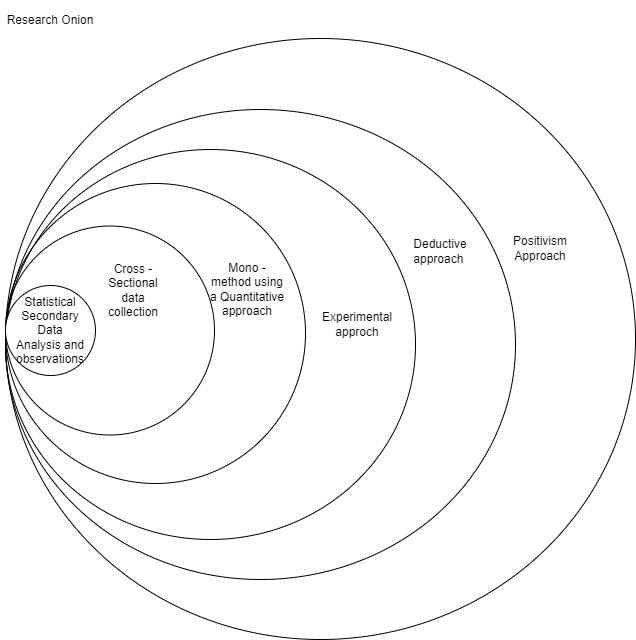
\includegraphics[width=\columnwidth]{./images/ResearhOnion.png}
    \caption{Research Onion}
    \label{fig:my_label}
\end{figure}

\begin{figure}[H]
    \centering
    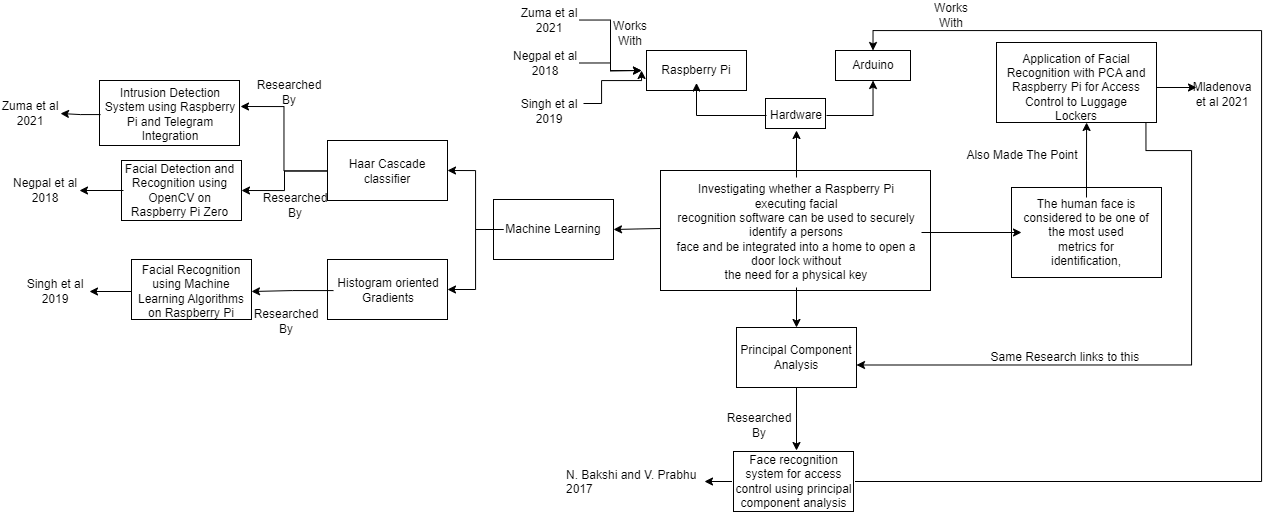
\includegraphics[width=\columnwidth]{./images/LiteratureMap.png}
    \caption{Research Onion}
    \label{fig:my_label}
\end{figure}
% use section* for acknowledgment
\section*{Acknowledgment}


The authors would like to thank...


% Can use something like this to put references on a page
% by themselves when using endfloat and the captionsoff option.
\ifCLASSOPTIONcaptionsoff
  \newpage
\fi



% trigger a \newpage just before the given reference
% number - used to balance the columns on the last page
% adjust value as needed - may need to be readjusted if
% the document is modified later
%\IEEEtriggeratref{8}
% The "triggered" command can be changed if desired:
%\IEEEtriggercmd{\enlargethispage{-5in}}

% references section

% can use a bibliography generated by BibTeX as a .bbl file
% BibTeX documentation can be easily obtained at:
% http://mirror.ctan.org/biblio/bibtex/contrib/doc/
% The IEEEtran BibTeX style support page is at:
% http://www.michaelshell.org/tex/ieeetran/bibtex/
%\bibliographystyle{IEEEtran}
% argument is your BibTeX string definitions and bibliography database(s)
%\bibliography{IEEEabrv,../bib/paper}
%
% <OR> manually copy in the resultant .bbl file
% set second argument of \begin to the number of references
% (used to reserve space for the reference number labels box)
\begin{thebibliography}{1}

\bibitem{IEEEhowto:kopka}
H.~Kopka and P.~W. Daly, \emph{A Guide to \LaTeX}, 3rd~ed.\hskip 1em plus
  0.5em minus 0.4em\relax Harlow, England: Addison-Wesley, 1999.

\end{thebibliography}

% biography section
% 
% If you have an EPS/PDF photo (graphicx package needed) extra braces are
% needed around the contents of the optional argument to biography to prevent
% the LaTeX parser from getting confused when it sees the complicated
% \includegraphics command within an optional argument. (You could create
% your own custom macro containing the \includegraphics command to make things
% simpler here.)
%\begin{IEEEbiography}[{\includegraphics[width=1in,height=1.25in,clip,keepaspectratio]{mshell}}]{Michael Shell}
% or if you just want to reserve a space for a photo:


% if you will not have a photo at all:

% You can push biographies down or up by placing
% a \vfill before or after them. The appropriate
% use of \vfill depends on what kind of text is
% on the last page and whether or not the columns
% are being equalized.

%\vfill

% Can be used to pull up biographies so that the bottom of the last one
% is flush with the other column.
%\enlargethispage{-5in}



% that's all folks
\end{document}


